\section{Experiments}
We conduct experiments on \textbf{ACE05} dataset,
which is a standard corpus for the entity relation extraction task.
It includes 7 entity types and 6 relation types between entities.
We use the same data split of ACE05 documents as previous work
(351 training, 80 development and 80 testing) \cite{miwa-bansal:2016:P16-1}.

We evaluate the performances using precision (P), recall
(R) and F1 scores following \cite{miwa-bansal:2016:P16-1,D18-1249}.
Specifically, an output entity $(e, y)$ is correct
if its type $y$ and the region of its head $e$ are correct, and an output
relation $r$ is correct if its $(e_1, y_1, e_2, y_2, l)$ are correct ( i.e., “exact match”).

In this paper, the default setting ``GCN'' is the 1-layer GCN-based joint model 
with the dynamic hard adjacency matrix, which achieves the best relation performance on ACE05 dataset.
\subsection{End-to-End Results on ACE05}



First, we compare proposed models with previous work in Table~\ref{tab:res-baseline-ace}.
In general,
our ``GCN''  achieves the best entity performance 84.2 percent
comparing with existing joint models.
For relation performance,
our ``GCN''  significantly outperforms all joint models 
except for \cite{D18-1249} which uses more complex joint decoder.
Comparing with our basic neural network ``NN'',
our ``GCN'' has large improvement both on entities and relations.
Those observations demonstrate the effectiveness of our ``GCN''  
for capturing information on multiple entity types and relation types from a sentence.

Compared to the state-of-the-art method which adopts minimum risk training \cite{D18-1249},
our ``GCN''   has better entity performance and comparable relation performance.
Different from existing joint decoding systems, 
we do not use complex joint decoding algorithms such as beam search \cite{li-ji:2014:P14-1}, 
global normalization \cite{zhang-zhang-fu:2017:EMNLP2017} and minimum risk training \cite{D18-1249}.
Our models only rely on sharing parameters similar to \cite{miwa-bansal:2016:P16-1,katiyar-cardie:2017:Long}.
It is worth noting that the precision of our ``GCN''  is
high compared to all the other methods. 
We attribute the phenomenon to the strong ability to model feature representations of entity nodes and relation nodes.
\begin{table}
\centering
\footnotesize
\begin{tabular}{l|lll|lll}
    \toprule
    \textbf{Model}&\multicolumn{3}{c}{\textbf{Entity}}&\multicolumn{3}{c}{\textbf{Relation}} \\
    & P & R & F & P & R & F\\
    \midrule
    L\&J \citeyearpar{li-ji:2014:P14-1} & 
    85.2 & 76.9 & 80.8 & 65.4 & 39.8 & 49.5\\
   
    Zhang \citeyearpar{zhang-zhang-fu:2017:EMNLP2017} 
    & - & - & 83.5 & - & - & 57.5 \\
    Sun \citeyearpar{D18-1249} & 83.9 & 83.2 & 83.6 & 64.9 & \textbf{55.1} & \textbf{59.6} \\
    \midrule
    M\&B \citeyearpar{miwa-bansal:2016:P16-1} & 
    82.9 & \textbf{83.9} & 83.4 & 57.2 & 54.0 & 55.6 \\
    K\&C \citeyearpar{katiyar-cardie:2017:Long} & 
    84.0 & 81.3 & 82.6 & 55.5 & 51.8 & 53.6 \\
    NN & 
    85.7 & 82.1 & 83.9 & 65.6 & 50.7 & 57.2 \\
    GCN  & \textbf{86.1} & 82.4 & \textbf{84.2} & \textbf{68.1} & 52.3 & 59.1 \\
    \bottomrule
\end{tabular}
\caption{\small Results on the ACE05 test data.
\citet{li-ji:2014:P14-1} 
\citet{zhang-zhang-fu:2017:EMNLP2017} and
\citet{D18-1249} are joint decoding algorithms.
\citet{miwa-bansal:2016:P16-1} and \citet{katiyar-cardie:2017:Long}
are joint training systems without joint decoding.
``NN'' is our neural network model without GCN.
``GCN'' is dynamic hard GCN-based neural network.
We omit pipeline methods which underperform joint models
(see \cite{li-ji:2014:P14-1} for details).
}
\label{tab:res-baseline-ace}
\end{table}

Next, we evaluate our model with different settings.
As mentioned in Section \ref{section:ent-rel-graph},
we have three types of graph: ``GCN (static)'', ``GCN (dynamic + hard)'' and ``GCN (dynamic + soft)''.
The last three rows of Table \ref{tab:framework-abla} show their performances.
We have three observations regarding the Table \ref{tab:framework-abla}.

\begin{enumerate}[leftmargin=*, itemindent=1pc]
    \item Compared with ``Sun (NN)'' model which is the base neural network without minimum risk training \cite{D18-1249},
    our ``NN''  performs better 0.5 point on entities.
    % and performs within 0.6 point on relations.
    One reason might be the entity type model and the relation type model share
    more parameters (entity CNN+MLP parameters),
    while ``Sun (NN)''  only shares biLSTM hidden states.
    However,
    our ``NN''  performs within 0.6 point on relations.
    One possible reason might be that
    we do not use the features of output entity type for relation type classification.
    \item 
    After introducing  graph convolutional networks,
    all three GCN-based models improve performances of entity and relation.
    Specifically,
    The ``GCN (static)''  has been slightly improved on relations.
    The ``GCN (dynamic + soft)'' achieves 0.7 percent improvement on relations 
    and has the same entity performance.
    The ``GCN (dynamic + hard)'' improves
    the entity performance (0.4 percent) \footnote{
    In fact, the entity performance on the ACE05 test data 
    is hard to improve from past works \cite{miwa-bansal:2016:P16-1,zhang-zhang-fu:2017:EMNLP2017,D18-1249}. So it is a non-negligible improvement over existing state-of-the-art systems.}
    and achieves large improvement (1.9 percent) in relation performance.
    It is competitive with state-of-the-art model \cite{D18-1249}.
    These observations show that the proposed joint model is effective for the joint type inference on entities and relations,
    and also show the rationality of the proposed dynamic graph, as expected.

    \item The performances of the entity span and the binary relation  are close to all proposed models. 
    One possible reason is that there are more coarse-gained task.
    Effective features can be easily extracted for all models.
    It  is  worth  noting  that the performance in binary relation
    is not very good.
    Our dynamic graph relies on binary relation detection task.
    How to improve the performance of binary relation is still a hard question.
    We leave it as future work.
\end{enumerate}

\begin{table}
	\centering
	\footnotesize
	\begin{tabular}{l|lll}
		\toprule
		 & 1-layer & 2-layer & 3-layer \\
        \midrule
        \textbf{F1 of Entity Span} & 90.4 & 90.5 & \textbf{90.7}\\
        \textbf{F1 of Binary Relation} & 61.5 & \textbf{62.9} & 62.8 \\
        \textbf{F1 of Entity} & 81.6 & 82.1 & \textbf{82.2}  \\
        \textbf{F1 of Relation} & \textbf{53.8} & 53.5 & 53.6 \\
		\bottomrule
	\end{tabular}
	\caption{\small Results on the ACE05 development set with respect to the number of GCN layers.}
	\label{tab:ace-gcn-layers}
\end{table}


\begin{table*}
	\centering
	\footnotesize
	\begin{tabular}{l|lll|lll|lll|lll}
		\toprule
		\textbf{Model} & \multicolumn{3}{c}{\textbf{Entity}} & \multicolumn{3}{c}{\textbf{Relation}} &  \multicolumn{3}{c}{\textbf{Entity Span}} & \multicolumn{3}{c}{\textbf{Binary Relation}} \\
		& P & R & F & P & R & F & P & R & F & P & R & F \\
        \midrule
        Sun (NN) \citeyearpar{D18-1249} & 84.0 & \textbf{82.9} & 83.4 & 59.5 & \textbf{56.3} & 57.8 & - & - & - & - & - & - \\
        NN & 85.7 & 82.1 & 83.9 & 65.6 & 50.7 & 57.2 & \textbf{91.2} & 89.6 & 90.4 & - & - & - \\

        GCN (static) & 85.0 & 82.6 & 83.8 & 66.6 & 51.3 & 57.8 & 90.8 & \textbf{90.2} & \textbf{90.5} & - & - & - \\
        
        GCN (dynamic + soft)& 85.3 & 82.3 & 83.8 & 67.3 & 51.6 & 58.5 & 90.8 & \textbf{90.2} & \textbf{90.5} & 77.3 & \textbf{56.4} & 65.2 \\
        GCN (dynamic + hard)& \textbf{86.1} & 82.4 & \textbf{84.2} & \textbf{68.1} & 52.3 & \textbf{59.1} & \textbf{91.2} & 89.5 & 90.4 & \textbf{78.2} & 56.3 & \textbf{65.4} \\
		\bottomrule
	\end{tabular}
	\caption{\small Results on the ACE05 dataset in different settings.}
	\label{tab:framework-abla}
\end{table*}



Thirdly, we present the influences of the number of GCN layers (Table \ref{tab:ace-gcn-layers}).
We take the ``GCN (dynamic + hard)'' as a example.
In general, 
the performances on four tasks are insensitive to the number of GCN layers \footnote{
We focus on the performance of the end-to-end
relation extraction, so we select models 
by the relation extraction results. 
It is also possible to consider both the 
performances of the entity model and the relation model.
We leave the study of advanced model selection algorithms 
for future work.
\label{foot:model_sel}
}.
In particular,
the performances on entity span, entity and relation fluctuate at 1.0 points,
and the binary relation fluctuate at 1.4 points.
Interestingly, 
we find the one layer GCN achieves best relation performance
though the performances of other three tasks are not best. 
One possible reason is that the all models are closely related to each other. However, how they affect each other in this joint settings is still
an open question.

Forthly,
we examine the relation performance with respect to different the number of relations for each sentence (Figure \ref{fig:rel_num}).
In general,
our GCN-based models almost outperform ``NN'' when the number of relations is larger than 2.
It proves that the proposed GCN-based models are more suitable for handle
multiple relations in a sentence.
We think our method will perform better 
on the complex multiple relations dataset
which is very common in reality.

\begin{figure}
    \begin{center}
        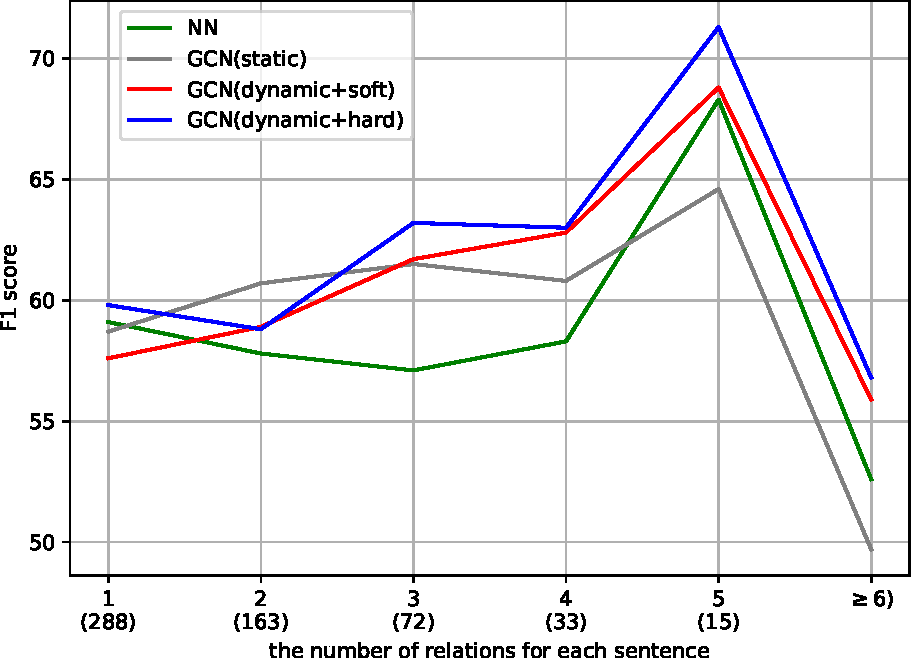
\includegraphics[width=2.8in]{../images/fig-rel-num.pdf}
    \end{center}
   \caption{F1 scores with respect to the number of relations for each sentence.
    The numbers in parentheses are counts of sentences in the ACE05 test set.}
    \label{fig:rel_num}
\end{figure}


%\begin{figure}
%    \begin{center}
%        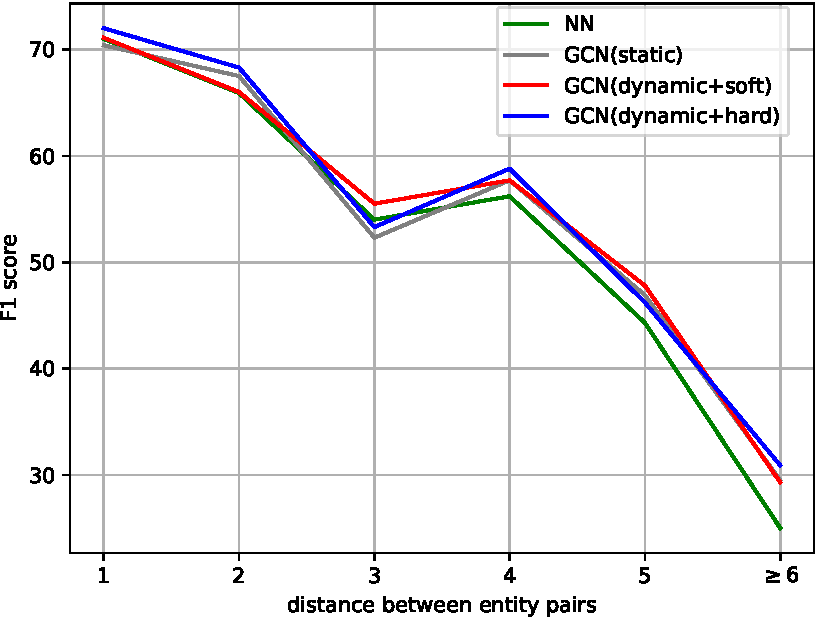
\includegraphics[width=3.0in]{../images/fig-distance.pdf}
%    \end{center}
%     \caption{F1 scores on ACE05 dataset with respect to the distance between entity pairs.}
%    \label{fig:len}
%\end{figure}


%Fifthly,
%we analysis the relation performance with respect to
%different distances between entity pairs (Figure \ref{fig:len}).
%Our GCN-based models achieve better performance for larger distance ($>3$).
%It shows that the GCN could capture some long distance dependency
%for joint extraction task.
%In addition,
%all models are not good at extracting relations over very long distances.
%Thus,  combining joint decoding algorithms
%with our model might be a promising direction in this joint extraction task.


Finally,
We compare the ``NN'' model with the ``GCN'' model
on some concrete examples, as shown in Table \ref{tab:case}.
For S1,
the ``NN'' wrongly identifies the relation \texttt{GEN-AFF} between 
``[legislature]\textsuperscript{\texttt{ORG}}'' and
``[north korea]\textsuperscript{\texttt{GPE}}''
even though the relation $\texttt{ORG-AFF}$ between 
``[legislature]\textsuperscript{\texttt{ORG}}'' and
``[chairman]\textsuperscript{\texttt{PER}}'' is detected.
For S2,
the ``NN'' does not detect \texttt{PART-WHOLE} relation 
while the ``GCN'' correctly find it.
These two observations show that our ``GCN'' is good at 
dealing with the situation 
when the multiple relations share common entities, as expected.
For S3,
our ``GCN'' identifies a \texttt{PHYS} relation between
``[units]\textsuperscript{\texttt{PER}}'' and
``[captial]\textsuperscript{\texttt{GPE}}'',
while the ``NN'' does not find this relation 
even the entities are correct.
However, both models do not identify the relation \texttt{ART} between
``[units]\textsuperscript{\texttt{PER}}'' and
``[weapons]\textsuperscript{\texttt{WEA}}''.
We think advanced improvement methods
which use more powerful graph neural network might be helpful
in this situation.


\subsection{Golden Entity Results on ACE05}
\begin{table}
	\centering
	\footnotesize
	\begin{tabular}{l|lll}
		\toprule
		\textbf{Model} & \multicolumn{3}{c}{\textbf{Relation}} \\
        \midrule
        M\&B \citeyearpar{miwa-bansal:2016:P16-1}  & \textbf{70.1} & 61.2 & 65.3  \\
        C\&M \citeyearpar{P18-2014} & 69.7 & 59.5 & 64.2 \\
        NN & 68.5 & 62.8 & 65.5 \\
     
        GCN (static) & 69.1 & 63.8 & 66.4 \\
        GCN (dynamic + soft)& 68.7 & 63.4 & 65.9 \\
        GCN (dynamic + hard)& 68.7 & \textbf{65.4} & \textbf{67.0}  \\
		\bottomrule
	\end{tabular}
	\caption{\small Results on the ACE05 dataset with golden entity.}
	\label{tab:ace-gold-entity}
\end{table}


In order to compare with relation classification methods,
we evaluate our models with golden entities on ACE05 corpus in Table \ref{tab:ace-gold-entity}.
We use the same data split to compare with their model \cite{miwa-bansal:2016:P16-1,P18-2014}.
We do not tune hyperparameters extensively. 
For example, we use the same setting in both end-to-end and golden entity
rather than tune parameters on each of them.
The baseline systems are \cite{miwa-bansal:2016:P16-1} and \cite{P18-2014}.

In general, 
our ``NN''  is competitive,
comparing to the dependency tree-based state-of-the-art model \cite{miwa-bansal:2016:P16-1}.
It shows that our CNN-based neural networks are able to extract
more powerful features to help relation extraction task.
After adding GCN,
our GCN-based models achieve the better performance.
This indicates that the proposed models can
achieve large improvement without any external syntactic tools
\footnote{For simplicity, we do not extract golden entity type features explicitly in our model.
And we believe there will be further improvements when these features are used.
}.

\begin{table*}
    \centering
    \renewcommand{\multirowsetup}{\centering}  
    \label{tab:err-1}
    % \vspace{0.2cm}
    \begin{tabular}{p{0.06\linewidth}|p{0.9\linewidth}}
        \toprule
        S1 & % however the firm announced on friday that it had reached a deal with 
        the 
        $\text{[british]}_{\texttt{GEN-AFF-2}: \heartsuit \clubsuit  \spadesuit}^{\texttt{GPE}:\heartsuit \clubsuit \spadesuit}$
        $\text{[arm]}_{\texttt{PART-WHOLE-1}: \heartsuit \spadesuit | \texttt{GEN-AFF-1}: \heartsuit \clubsuit \spadesuit}^{\texttt{ORG}:\heartsuit \clubsuit \spadesuit}$
        of french distributors 
        $\text{[pathe]}_{\texttt{PART-WHOLE-2}: \heartsuit \spadesuit}^{\texttt{ORG}:\heartsuit \clubsuit \spadesuit}$
        to show four releases . 
        \\
        \bottomrule
    \end{tabular}
    
    \label{tab:err-2}
    % \vspace{0.2cm}
    \begin{tabular}{p{0.06\linewidth}|p{0.9\linewidth}}
        \toprule
        S2 &
        %during their visit to pyongyang , weldon 's delegation also met choe thae bok , 
        \dots
        $\text{[chairman]}_{\texttt{ORG-AFF-1}: \heartsuit \clubsuit \spadesuit}^{\texttt{PER}:\heartsuit \clubsuit \spadesuit}$
        of 
        $\text{[north korea ]}_{\texttt{PART-WHOLE-2}: \heartsuit \spadesuit | \texttt{GEN-AFF-2}: \clubsuit}^{\texttt{GPE}:\heartsuit \clubsuit \spadesuit}$
        's 
        $\text{[legislature]}_{\texttt{PART-WHOLE-1}: \heartsuit \spadesuit| \texttt{ORG-AFF-2}: \heartsuit \clubsuit \spadesuit | \texttt{GEN-AFF-1}: \clubsuit}^{\texttt{ORG}:\heartsuit \clubsuit \spadesuit}$
        , the supreme people  's assembly .    
        \\
        \bottomrule
    \end{tabular}
    \label{tab:err-3}
    \begin{tabular}{p{0.06\linewidth}|p{0.9\linewidth}}
        \toprule
        S3 & 
         % u.s. officials say some intelligence indicates 
         a red line may have been drawn around the 
        $\text{[capital]}_{\texttt{PHYS-2}: \heartsuit \spadesuit}^{\texttt{GPE}:\heartsuit \clubsuit \spadesuit}$ 
        with 
        $\text{[republican gurad]}_{\texttt{ORG-AFF-2}: \heartsuit \clubsuit \spadesuit}^{\texttt{ORG}:\heartsuit \clubsuit \spadesuit} $
        $\text{[units]}_{\texttt{PHYS-1}: \heartsuit \spadesuit| \texttt{ORG-AFF-1}: \heartsuit \clubsuit \spadesuit| \texttt{ART-1}: \heartsuit}^{\texttt{PER}:\heartsuit \clubsuit \spadesuit} $
        ordered to use chemical 
        $\text{[weapons]}_{\texttt{ART-2}: \heartsuit}^{\texttt{WEA}:\heartsuit \clubsuit \spadesuit} $
        once u.s. and allied troops cross it .
        \\
        \bottomrule
    \end{tabular}
    \caption{Examples from the ACE05 dataset
    with label annotations from ``NN'' model and ``GCN'' model
    for comparison. 
    The $\heartsuit$ is the gold standard,
    and the $\clubsuit$, $\spadesuit$ are the output of the ``NN'' 
    ,``GCN'' model respectively.}
    \label{tab:case}
\end{table*}


